\chapter{lineær programmering}

Lineær programmering er en anvendelse af lineær algebra til at finde den optimale resultat af et optimeringsproblem. Lineære programmeringsproblemer tager udgangspunkt i maksimering eller minimering af en lineær funktion. For variablene er der fastsat en række af betingelser, som begrænser de mulige løsninger til problemet.



Funktionen, som ønskes optimeret, kaldes \textbf{kriteriefunktionen}, og findes på formen:
\begin{align}
f(x_1,x_2,\cdots , x_n)\ =\ c_1x_1 + c_2x_2 + \cdots + c_nx_n.
\end{align}

Dertil tilføjes en række af betingelser for variablene. Betingelser, som definerer at en variabel er positiv, kaldes en \textbf{positivitetsbetingelse}. 
\begin{align}
	x_i \geq 0
\end{align}
Andre lineære betingelser for variablene kaldes for \textbf{lineære bibetingelser}, og findes på formen, 
\begin{align}
	a_{i,1} x_1 + a_{i,2} x_2 + \cdots + a_{i,n} x_n \leq b_i, \quad \text{for} \ i \in \{1,2,\cdots, m\},
\end{align}
hvor $m$ er antallet af lineære bibetingelser. I en lineær bibetingelse kan venstresiden være begrænset med $\leq, \geq,<,>$ eller $=$ i forhold til konstanten $b_i$. I nogle typer af programmeringsproblemer anvendes kun en enkelt af disse relationer. Positivitetsbetingelser er et specialtilfælde af de lineære bibetingelser.

En \textbf{løsning} til et lineært programmeringsproblem betegner værdier af variablene, som overholder alle betingelserne.

Et eksempel på et lineært programmeringsproblem ses i Eksempel \ref{eks:maksprob1}. Eksemplet er et lineært maksimeringsproblem, da objektfunktionen søges maksimeret.

\begin{eks}
Et eksempel på et lineært programmeringsproblem ses her, hvor funktionen $f(x_1,x_2)=4x_1+3 x_2$ skal maksimeres.
\begin{center}
\begin{tabular}{l	>{$}r<{$}	>{$}r<{$}	>{$}l<{$}}
Maksimer 		& 4x_1&		+3 x_2& \\
med hensyn til 	& - \ \ x_1& 	+4 x_2& \leq 12\\
				&  x_1& 	+2 x_2& \leq 12\\
				&- \ \ x_1& 	+ \ \ x_2& \geq -6\\
og $x_2\geq 0$
\end{tabular}
\end{center}

Mængden af alle mulige løsninger til problemet kan vises grafisk. De mulige løsninger findes inden for det grå område på Figur \ref{fig:maksprob1}, hvor $x_1$ og $x_2$ vises henholdsvist på 1. og 2. aksen.

\begin{center}
	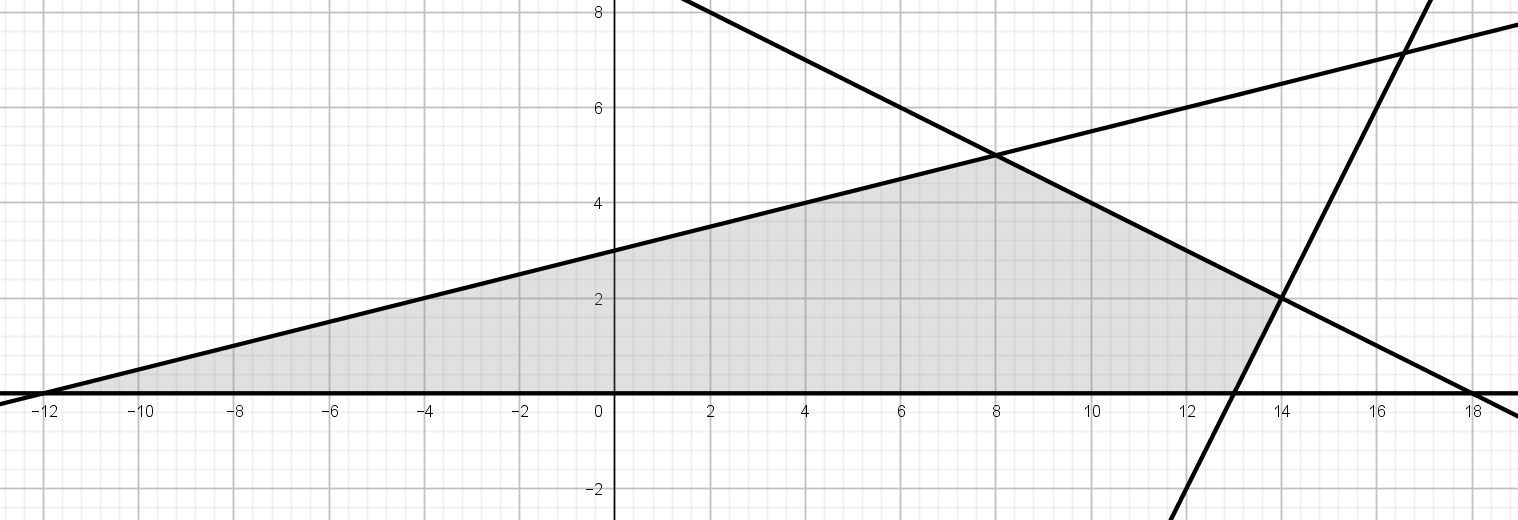
\includegraphics[scale=0.2]{fig/prog/feasibleset1}
	\captionof{figure}{Den mulige mængde (bør laves til tikz)}
	\label{fig:maksprob1}
\end{center}
\label{eks:maksprob1}
\end{eks}

\section{Standard maksimums- og minimumsproblemer}
I et standard maksimumsproblem gælder det for alle bibetingelserne at den lineære funktion af variablene er mindre end eller lig en konstant, samt at alle variablene er positivt begrænsede.

Som beskrevet i Afsnit \ref{afsnit:lign_sys} kan et lineært ligningssystem opskrives som et matrix-vektor produkt. Tilsvarende gælder det for kriteriefunktionen, at denne kan skrives som et produkt af to vektorer. Det tillader derved definitionen af standard maksimum problemet med disse produkter i definition \ref{def:std_maks}

\begin{defn}[Standard maksimum problem]
	Lad $\vec{x}= [x_1, x_2,\cdots, x_n]^T$ være \textbf{løsningsvektoren}, med koefficienter $\vec{c}= [c_1, c_2,\cdots, c_n]^T$ i kriteriefunktionen, og lad $mxn$ matrixen $A=[A_{ij}]$ for $i=1,2,\cdots,m$ og $j=1,2,\cdots,n$ være begrænset af konstanterne $\vec{b}=[b_1, b_2,\cdots, b_m]^T$.
	Da er standard maksimum problemet defineret som\\
\begin{center}
\begin{tabular}{l	>{$}l<{$}}
Maksimer 		& \vec{c}^T\vec{x} \\
med hensyn til 	& A\vec{x} \leq \vec{b}\\
og 				& \vec{x} \geq \vec{0}
\end{tabular}
\end{center}
\label{def:std_maks}
\end{defn}

\begin{defn}[Standard minimum problem]
	Lad $\vec{y}= [y_1, y_2,\cdots, y_m]^T$ være \textbf{løsningsvektoren}, med koefficienter $\vec{b}= [b_1, b_2,\cdots, b_m]^T$ i kriteriefunktionen, og lad $mxn$ matrixen $A=[A_{ij}]$ for $i=1,2,\cdots,m$ og $j=1,2,\cdots,n$ være begrænset af konstanterne $\vec{c}=[c_1, c_2,\cdots, c_n]^T$.
	Da er standard minimum problemet defineret som\\
\begin{center}
\begin{tabular}{l	>{$}l<{$}}
Minimer			& \vec{y}^T\vec{b} \\
med hensyn til 	& \vec{y}^TA \geq \vec{c}^T\\
og 				& \vec{y} \geq \vec{0}
\end{tabular}
\end{center}
\label{def:std_min}
\end{defn}

\begin{eks}
Hvis eksempel \ref{eks:maksprob1} skal omskrives til et standard maksimum problem, skal ale uligheder i bibetingelserne være $\leq$. Bibetingelse nr.3 skal derved omskrives. Dette kan gøres ved at gange begge sider af uligheden med $-1$, da dette vender ulighedstegnet. Derudover skal også $x_1$ skal være positivt begrænset. Derved bliver Eksempel \ref{eks:maksprob1} omskrevet til et standard maksimum problem til\\
\begin{center}
\begin{tabular}{l	>{$}r<{$}	>{$}r<{$}	>{$}l<{$}}
Maksimer 		& 4x_1&		+3 x_2& \\
med hensyn til 	& - \ \ x_1& 	+4 x_2& \leq 12\\
				&  x_1& 	+2 x_2& \leq 12\\
				&  x_1& 	-\ \ x_2& \geq 6\\
og $x_1 \geq 0, x_2\geq 0$.
\end{tabular}
\end{center}
\end{eks}

\section{Løsninger til linære programmeringsproblemer}

Den mulige løsningsmængde 

\begin{defn}[Mulige løsninger og løsningsmængden]
En \textbf{mulig løsning} er en løsningsvektor $\vec{x}$, som opfylder alle problemets betingelser.\\
\textbf{Løsningsmængden} $\mathds{F}$ \textit{(usikker på oversættelsen)} er mængden af alle de mulige løsninger.
En vektor $\vec{x}$ kaldes en \textbf{optimal løsning}, hvis $f(\vec{x})=\max\limits_{x \in \mathds{F}}f(\vec{x}).$
\end{defn}

\begin{comment}
Hvad skal med i dette afsnit?
- hvad betyder lineær programmering.
	en måde at anvende lineær algebra til at løse nogle forskellige problemer, hvor det gælder om at optimere et resultat.
	I et lineært programmeringsproblem er der en funktion, kaldet den objektive funktion, som forsøges optimeret.
	for et sådan problem er der fastsat en række begrænsninger. 
	fælles for den objektive funktion og begrænsningerne er at de alle er lineære funktioner. 
	
Objektfunktionen findes derved på formen:
$ F: \mathds{R}^n \rightarrow \mathds{R} 
$ hvor n er antallet af variable, som indgår i problemet.

Kriteriefunktionen er en lineær funktion af indgangene i vektoren $\vec{x}$.

Bibetingelserne findes på formen:
$\vec{a}$
\end{comment}